\documentclass{standalone}
\usepackage{tkz-fct}
\usepackage{tkz-euclide}
\usepackage{color}
\renewcommand*\familydefault{\sfdefault}
\usepackage{sansmath}
\sansmath
\definecolor{gray75}{gray}{0.75}
\begin{document}
 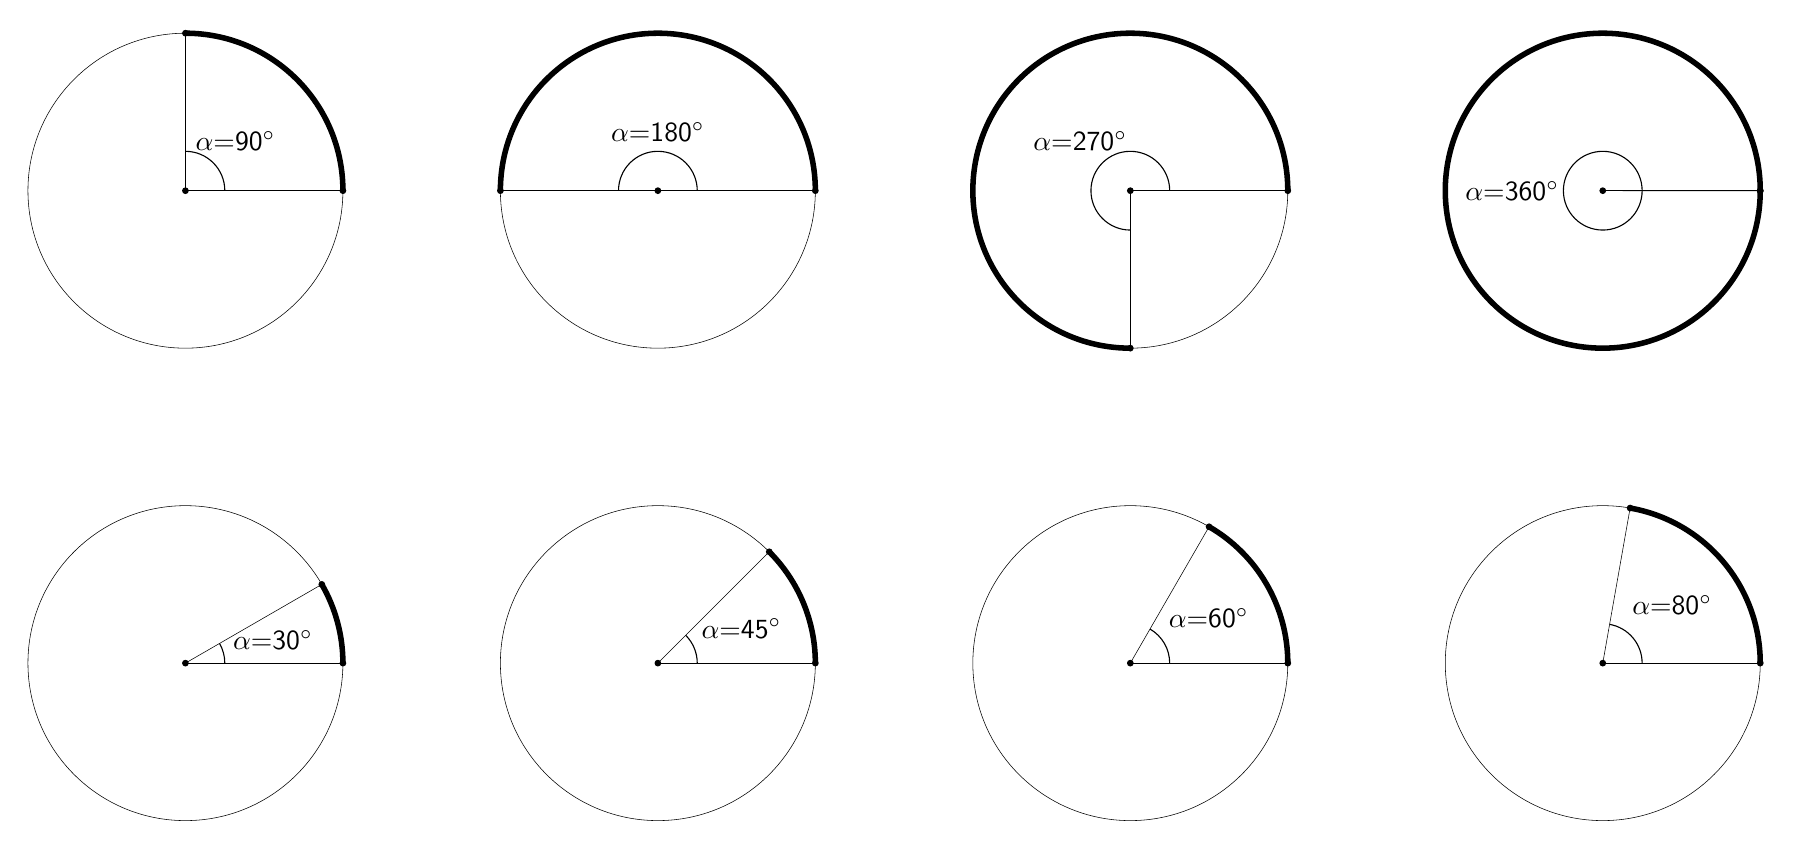
\begin{tikzpicture}[scale=2]

   \tkzDefPoints{0/0/O,1/0/A}
   \tkzDrawCircle[color=black](O,A)
   \tkzDefPointBy[rotation= center O angle 90](A)
   \tkzGetPoint{B}
   \tkzDrawSegment(O,A)
   \tkzDrawSegment(O,B)
   \tkzDrawArc[color=black,line width=2pt](O,A)(B)
   \tkzDrawPoints(A,B,O)
   \tkzPicAngle["$\alpha$=90$^{\circ}$",draw=black,
-,angle eccentricity=1.8,
angle radius=0.5cm](A,O,B)
\begin{scope}[xshift=3cm]
\tkzDefPoints{0/0/O,1/0/A}
   \tkzDrawCircle[color=black](O,A)
   \tkzDefPointBy[rotation= center O angle 180](A)
   \tkzGetPoint{B}
   \tkzDrawSegment(O,A)
   \tkzDrawSegment(O,B)
   \tkzDrawArc[color=black,line width=2pt](O,A)(B)
   \tkzDrawPoints(A,B,O)
   \tkzPicAngle["$\alpha$=180$^{\circ}$",draw=black,
-,angle eccentricity=1.5,
angle radius=0.5cm](A,O,B)
\end{scope}
\begin{scope}[xshift=6cm]
\tkzDefPoints{0/0/O,1/0/A}
   \tkzDrawCircle[color=black](O,A)
   \tkzDefPointBy[rotation= center O angle 270](A)
   \tkzGetPoint{B}
   \tkzDrawSegment(O,A)
   \tkzDrawSegment(O,B)
   \tkzDrawArc[color=black,line width=2pt](O,A)(B)
   \tkzDrawPoints(A,B,O)
   \tkzPicAngle["$\alpha$=270$^{\circ}$",draw=black,
-,angle eccentricity=1.8,
angle radius=0.5cm](A,O,B)
\end{scope}
\begin{scope}[xshift=9cm]
\tkzDefPoints{0/0/O,1/0/A}
   \tkzDrawCircle[color=black](O,A)
   \tkzDefPointBy[rotation= center O angle 359.9](A)
   \tkzGetPoint{B}
   \tkzDrawSegment(O,A)
   \tkzDrawSegment(O,B)
   \tkzDrawArc[color=black,line width=2pt](O,A)(B)
   \tkzDrawPoints(A,B,O)
   \tkzPicAngle["$\alpha$=360$^{\circ}$",draw=black,
-,angle eccentricity=2.3,
angle radius=0.5cm](A,O,B)
\end{scope}
\begin{scope}[yshift=-3cm]
   \tkzDefPoints{0/0/O,1/0/A}
   \tkzDrawCircle[color=black](O,A)
   \tkzDefPointBy[rotation= center O angle 30](A)
   \tkzGetPoint{B}
   \tkzDrawSegment(O,A)
   \tkzDrawSegment(O,B)
   \tkzDrawArc[color=black,line width=2pt](O,A)(B)
   \tkzDrawPoints(A,B,O)
   \tkzPicAngle["$\alpha$=30$^{\circ}$",draw=black,
-,angle eccentricity=2.3,
angle radius=0.5cm](A,O,B)
\begin{scope}[xshift=3cm]
\tkzDefPoints{0/0/O,1/0/A}
   \tkzDrawCircle[color=black](O,A)
   \tkzDefPointBy[rotation= center O angle 45](A)
   \tkzGetPoint{B}
   \tkzDrawSegment(O,A)
   \tkzDrawSegment(O,B)
   \tkzDrawArc[color=black,line width=2pt](O,A)(B)
   \tkzDrawPoints(A,B,O)
   \tkzPicAngle["$\alpha$=45$^{\circ}$",draw=black,
-,angle eccentricity=2.3,
angle radius=0.5cm](A,O,B)
\end{scope}
\begin{scope}[xshift=6cm]
\tkzDefPoints{0/0/O,1/0/A}
   \tkzDrawCircle[color=black](O,A)
   \tkzDefPointBy[rotation= center O angle 60](A)
   \tkzGetPoint{B}
   \tkzDrawSegment(O,A)
   \tkzDrawSegment(O,B)
   \tkzDrawArc[color=black,line width=2pt](O,A)(B)
   \tkzDrawPoints(A,B,O)
   \tkzPicAngle["$\alpha$=60$^{\circ}$",draw=black,
-,angle eccentricity=2.3,
angle radius=0.5cm](A,O,B)
\end{scope}
\begin{scope}[xshift=9cm]
\tkzDefPoints{0/0/O,1/0/A}
   \tkzDrawCircle[color=black](O,A)
   \tkzDefPointBy[rotation= center O angle 80](A)
   \tkzGetPoint{B}
   \tkzDrawSegment(O,A)
   \tkzDrawSegment(O,B)
   \tkzDrawArc[color=black,line width=2pt](O,A)(B)
   \tkzDrawPoints(A,B,O)
   \tkzPicAngle["$\alpha$=80$^{\circ}$",draw=black,
-,angle eccentricity=2.3,
angle radius=0.5cm](A,O,B)
\end{scope}
\end{scope}

\end{tikzpicture}
\end{document}
